\documentclass[12pt,smallheadings, bibliography=totoc]{scrartcl}
%\setkomafont{caption}{\small\bfseries\selectfont}
%\setkomafont{captionlabel}{\small\bfseries}
\usepackage[headsepline,automark]{scrlayer-scrpage} %Trennlinie an Kopfzeile
%\usepackage{scrheadings}
\clearpairofpagestyles
\lohead{\rightmark}
%\renewcommand{\partmark}[1]{\relax}% \part daran hindern, den Kolumnentitel zu löschen
\ohead[]{\pagemark}
%\ofoot*{\pagemark}
%%Kopfzeile
\usepackage{txfonts} %für times new roman
%\usepackage{helvet} %für arial, dann aber 11pt
\usepackage[a4paper, left=2cm, right=2.5cm]{geometry}
\usepackage[onehalfspacing]{setspace}
%\usepackage{apacite}
\usepackage{caption}
\captionsetup{labelfont={footnotesize,bf}}
\captionsetup{font={footnotesize,bf}}
\usepackage{wasysym}
\usepackage{mbenotes}
\usepackage{rotating}
\usepackage{framed}
%\usepackage{amsmath}
%\usepackage{amssymb}
\usepackage{float}
%\usepackage{caption}
\usepackage[T1]{fontenc}
\usepackage[utf8]{inputenc}
%\usepackage{todonotes}
\usepackage{enumitem}
%\uespackage{caption}
%\usepackage[bf]{caption}
%\renewcommand{\captionfont}{\small\slshape}
%\renewcommand{\figurename}{Abb.}
%\renewcommand{\thefigure}{\arabic{section}.\arabic{figure}}
%\makeatletter \@addtoreset{figure}{section} \makeatother
%\captionsetup[figure]{skip=1pt}
\usepackage{tabularx}
\usepackage{hfoldsty}
\usepackage[osf,sc]{mathpazo}
\usepackage{pdfpages}
\usepackage{array}
\usepackage{hyperref}
\usepackage{threeparttable} %fußnoten unterhalb tabelle
\usepackage{booktabs} % fuer schone Tabellen
\usepackage{rotating} % um tabellen auf quer drehen zu koennen http://www.golatex.de/kann-man-tabellen-im-querformat-darstellen-t2003.html
%\newcolumntype{C}[1]{>{\centering\arraybackslash}p{#1}} %Spalten mit fester breite zentriert
%\newcolumntype{L}[1]{>{\raggedright\arraybackslash}p{#1}} %Spalten mit fester breite linksbündig
%\newcolumntype{Y}{>{\small\raggedright\arraybackslash}X}
%\newcolumntype{C}{>{\small\centering\arraybackslash}X}
\usepackage{graphicx}
%\usepackage[german]{babel}
\usepackage{typearea}
%für Randbemerkungen, sehr nützlich:
\usepackage{xargs}                      % Use more than one optional parameter in a new commands
\usepackage[pdftex,dvipsnames]{xcolor}
\usepackage[colorinlistoftodos,prependcaption,textsize=tiny]{todonotes}
\newcommandx{\unsure}[2][1=]{\todo[linecolor=red,backgroundcolor=red!25,bordercolor=red,#1]{#2}}
\newcommandx{\change}[2][1=]{\todo[linecolor=blue,backgroundcolor=blue!25,bordercolor=blue,#1]{#2}}
\newcommandx{\info}[2][1=]{\todo[linecolor=OliveGreen,backgroundcolor=grenn!25,bordercolor=OliveGreen,#1]{#2}}
\newcommandx{\improvement}[2][1=]{\todo[linecolor=Plum,backgroundcolor=orange!25,bordercolor=Plum,#1]{#2}}
\newcommandx{\thiswillnotshow}[2][1=]{\todo[disable,#1]{#2}}
% erklaerung siehe hier http://tex.stackexchange.com/questions/9796/how-to-add-todo-notes

%hat prima funktioniert:
\usepackage[style=apa,backend=biber]{biblatex}
\usepackage[american,ngerman]{babel}
\DeclareLanguageMapping{ngerman}{ngerman-apa}
\usepackage[babel,german=guillemets]{csquotes}
%\bibliographystyle{apacite}
%nach part fängt section wieder mit eins an alte Gestaltung
%\makeatletter
%\@addtoreset{section}{part}
%\makeatother
%\renewcommand*{\partformat}{\thepart}{}
%\renewcommand*{\partheadmidvskip}{\nobreak\enskip}
\bibliography{/Users/Mama/Dropbox/Biblio/library}
%\bibliography{/Users/iNge/Dropbox/Biblio/library}
%\bibliography{library}




\begin{document}
\renewcommand\finalandcomma{\addcomma}

\begin{titlepage}
\thispagestyle{empty}
\begin{center}
\Large{Fernuniversität Hagen}\\
\end{center}


\begin{center}
%\Large{Bildung und Medien: eEducation}
\end{center}
\begin{verbatim}



\end{verbatim}
\begin{center}
\textbf{\Large{Evaluation der Lernumgebung: „Umsetzung des Bildungs- Orientierungsplans mit dem Early Excellence-Konzept“}}
\end{center}
\begin{verbatim}

\end{verbatim}
\begin{center}
\textbf{Fakultät Kulturwissenschaften}
\end{center}
\begin{verbatim}




\end{verbatim}

\begin{flushleft}
\begin{tabular}{lll}
\textbf{Studiengang:} & & MA Bildung und Medien: eEducation\\
& & Modul 2: (Anwendungsbezogene) Bildungsforschung\\
& & \\
& & \\
\textbf{eingereicht von:} & & {Inge Koch-Meinass \\
& & {Matrikelnr.: 965092}\\
& & \\
\textbf{eingereicht am:} & & 01. April 2016\\
& & \\
& & \\
\textbf{Betreuer:} & & Dr. Boris Becker\\ & & Anne Martin \\ & & Burkhard Raue
\end{tabular}
\end{flushleft}

% das ist wohl jetzt das Ende des Dokumentes
\end{titlepage}


%% das Papierformat zuerst
%\documentclass[a4paper, 11pt]{article}

% deutsche Silbentrennung
%\usepackage[ngerman]{babel}
%\usepackage{color} \color{blue}
% wegen deutschen Umlauten
%\usepackage[utf8]{inputenc}

% hier beginnt das Dokument
%\begin{document}

\begin{titlepage}
\thispagestyle{empty}
\begin{center}
\color{blue}\Large{Fernuniversität Hagen}\\
\end{center}


\begin{center}
%\Large{Bildung und Medien: eEducation}
\end{center}
\begin{verbatim}



\end{verbatim}
\begin{center}
\textbf{\Large{Kommentierte Bibliographie zum Thema Online-Lernen}}
\end{center}
\begin{verbatim}

\end{verbatim}
\begin{center}
%\textbf{im Studiengang Wirtschaftsinformatik}
\end{center}
\begin{verbatim}











\end{verbatim}

\begin{flushleft}
\begin{tabular}{lll}
\textbf{Studiengang:} & & MA Bildung und Medien: eEducation\\
& & Modul 2: Anwendungsbezogene Bildungsforschung\\
& & \\
& & \\
\textbf{eingereicht von:} & & {\color{magenta} Inge Koch-Meinass \flq{}ingekoch@mac.com\frq{}}\\
& & {\color{magenta}Matrikelnr.: 9650962 }\\
& & \\
\textbf{eingereicht am:} & & 06. November 2015\\
& & \\
& & \\
%\textbf{Betreuer:} & & Herr Prof. Dr. J. A. Müller
\end{tabular}
\end{flushleft}

% das ist wohl jetzt das Ende des Dokumentes
\end{titlepage}

\pagenumbering{Roman}
\listoftodos[Gesammelte Unklarheiten]
\tableofcontents
\listoftables
\listoffigures
%\setcounter{page}{1}
%\thispagestyle{empty}
\clearpage
\pagebreak
\pagenumbering{arabic}
\section{Einleitung}\label{einleitung}

\glqq Das weltweit verfügbare Wissen verdoppelt sich zurzeit alle vier
bis fünf Jahre. Der amerikanische Soziologe Richard Sennet (1998)
erwartet, dass ein amerikanischer College Student in seinem Berufsleben
elf Mal die Stelle wechselt und dreimal die Basis seines Wissens
komplett austauscht \parencite[138]{Ehlers2002}.\grqq{} Vor diesem
Hintergrund kommt der beruflichen Weiterbildung eine immer größere
Bedeutung zu, den beruflichen Anforderung gerecht zu werden, erfordert
die Bereitschaft zu lebenslangem Lernen. Mit dem Zuwachs an Veränderung
in Organisationen und der damit verbundenen Anforderung „am Ball zu
bleiben`` gilt es Lernkonzepte zu finden, die modernen,
konstruktivistischen Lerntheorien einerseits und beruflichem Lernen von
Erwachsenen andererseits gerecht werden. Das immer größere Lernpensum
kann nicht mehr ausschließlich in Präsenzveranstaltung gelehrt werden,
es ist daher notwendig von Zeit und Ort unabhängige Lernmöglichkeiten zu
schaffen. Digitale Lernplattformen leisten hier einen wichtigen Beitrag
und können je nach didaktischer Aufbereitung, selbstorganisiertes,
konstruktivistisches und damit nachhaltiges Lernen fördern
\parencite{Kerres2002}. Die vorliegende Arbeit befasst sich mit der
Evaluation einer beruflichen Weiterbildung, die als Blended Learning
Kurs für
Frühpädagoginnen\footnote{Der Begriff Frühpädagogin, schließt alle im Kitabereich tätigen Fachkräfte ein}\footnote{Aus Gründen der besseren Lesbarkeit wird hier jeweils nur die weibliche, die männliche oder die geschlechtsneutrale Bezeichnung verwendet. Personen aller Geschlechter sind gleichermaßen einbezogen}
konzipiert wurde. Inhalt der Weiterbildung ist das Kennenlernen und
Umsetzen des Early-Excellence Konzeptes (EEC), ein Ansatz mit dem
Bildungs- und Orientierungspläne der Bundesländer in den
Kindertagesstätten konzeptionell verankert werden können. Mit Hilfe
eines standardisierten Fragebogens wird versucht, den durch die
Weiterbildung gewonnenen, selbst eingeschätzten Zuwachs an
Handlungskompetenz zu bestimmen. Es wird einmal das
Weiterbildungsangebot insgesamt und zum anderen der Einfluss der
digitalen Lernplattform betrachtet.

\section{Theorierahmen}\label{theorierahmen}

Der der Untersuchung zugrundeliegende Theorierahmen umfasst die Themen
Erwachsenenbildung im Blended Learning Verfahren und daraus
resultierender Zuwachs an Handlungskompetenz.

\subsection{Erwachsenenbildung}\label{erwachsenenbildung}

Das Lernen Erwachsener unterliegt besonderen Gegebenheiten, die hier
nachfolgenden beschrieben werden. Lernen im Erwachsenenalter ist
überwiegend gekennzeichnet durch Anschlusslernen. Der Erwachsene knüpft
beim Lernen an Bekanntes an, Lernen erfolgt konstruktivistisch und
subjektorientiert: „Erwachsene lassen sich in der Regel nicht belehren
oder aufklären, Wahrheiten lassen sich nicht linear vermitteln.
Erwachsene haben ihren eigenen Kopf, machen sich ihre eigenen
Gedanken\ldots`` \parencite[15]{Siebert201408}. Dies unterstreicht
einmal mehr, dass Lernen nicht hergestellt, sondern nur vom Individuum
selbst vollbracht werden kann \parencite{Faulstich2012}.

In subjektorientierten Lerntheorien z.B.: \parencite{Holzkamp2004} wird
Lernen beschrieben als eine Erweiterung von Handlungsfähigkeit und nicht
als Anhäufung von Wissen. Holzkamp prägte den Begriff des „expansiven
Lernens'', der ausdrücken soll, dass „intentionales, d.h. absichtliches
und geplantes Lernen nur dann zustande kommt, wenn das Lernsubjekt
selbst entsprechende Gründe dafür hat`` {[}\ldots{]}
\parencite[29]{Holzkamp2004}. Nach Holzkamp kommt es dann zum Lernen,
wenn das „Subjekt in seinem normalen Handlungsvollzug auf Hindernisse
oder Widerstände gestoßen ist{[}\ldots{]}.`` Im vorliegenden Fall ist
das „Hindernis`` die Einführung von Bildungs- und Orientierungsplänen in
Kitas, die es erforderlich machen den „normalen Handlungsvollzug`` zu
verändern. Diese Problematik kann nicht mit dem vorhandenen Wissen und
den vorhandenen Fähigkeiten gelöst werden, sondern erfordert das
„Einschalten einer Lernschleife`` \parencite[29]{Holzkamp2004}. Diese
Lernschleife wird mit der hier beschriebenen Weiterbildungsmaßnahme,
unter Berücksichtigung, dass es unmöglich ist, Inhalte passiv in Köpfe
füllen zu können \parencite[12]{Faulstich2012}, gedreht. Schon 1993
verweist Holzkamp in seinem Buch „Lernen`` auf die Notwendigkeit, den
Lerner in den Mittelpunkt zu stellen, verweist auf den
Lehr-Lern-Kurzschluss\footnote{Hiermit ist gemeint, dass nicht alles was gelehrt wird, auch gelernt wird}
und übt scharfe Kritik am vorherrschenden Schulsystem. Während die
didakische Umsetzung der Subjektorientierung in Schulen wenig
aufgegriffen wird, ist sie in der beruflichen Erwachsenenbildung eher
gängig \parencite{grotluschen2005expansives}.
\textcite[138]{ehlers2011qualitat} beschreibt vier Gründe für den immer
größer werdenden Stellenwert des Lerners in Weiterbildungsmaßnahmen:
\emph{Ökonomische} Gründe liegen vor, weil die Lerner Weiterbildung oft
selbst finanzieren und/oder die Weiterbildung in der Freizeit machen.
\emph{Pädagogisch-didaktische} Gründe liegen im Wandel zu
konstruktivistischen Lerntheorien, die eine Subjektorientierung
bedingen. \emph{Gesellschaftlich} ist die Entwicklung hin zur
Wissensgesellschaft zu betrachten und die Entwicklung hin zum
\emph{eLearning} als Lernform, dass per se den Lerner als Akteur
einbezieht. Auch die hier beschriebene Weiterbildungsmaßnahme orientiert
sich an den Grundlagen des subjektorientierten Lernens und vor dem
Hintergrund, dass die Teilnehmer sehr individuelle Lernzugänge haben und
letztlich nur selbst ihre Handlungsfähigkeit erweitern können. Die
Inhalte bestehen weniger in Vermittlung von Faktenwissen, als vielmehr
in der Anknüpfung von bereits Erlebten in Form von Biographiearbeit und
der Berücksichtigung der jeweils unterschiedlichen Kontextbezügen. Dies
wird in den Präsenzphasen, als auch mit der Lernplattform beispielsweise
dadurch umgesetzt, dass die Lerner zugleich auch Lehrende sind, Inhalte
aktiv mitgestalten und wiederum der Gemeinschaft zur Verfügung stellen.

Vor diesem Hintergrund wird in der vorliegenden Arbeit der „Lernerfolg``
eben als solche Erweiterung von Handlungsfähigkeit, in Form von Zuwachs
an Handlungskompetenz gemessen.

\subsection{Blended Learning}\label{blended-learning}

Im folgenden soll der Begriff des Blended Learning und was im Rahmen
dieser Arbeit darunter zu verstehen ist, erläutert werden. Direkt
übersetzt bedeutet Blended Lerning „vermischtes Lernen``. Das heißt es
handelt sich bei dieser Lernform um ein Lehr-Lernsetting, dass sowohl
klassisches Face-to-Face-Lernen, als auch eLearning beinhaltet. Die
verschiedenen Lernangebote stehen sich nicht als entweder oder
gegenüber, sondern als sich ergänzend.
\textcite[3]{kerres2001multimediale} betont „dass die besondere Qualität
und auch Effizienz eines Lernangebotes vor allem in der Kombination von
Elementen unterschiedlicher methodischer und medialer Aufbereitung zum
Tragen kommt``. \textcite[45]{ehlers2011qualitat} merkt kritsch an, dass
der Begriff nicht vermischtes Lernen meint, sondern, dass es um eine
Mischung von Methoden mit denen gelernt wird, geht. „Blended Learning
strebt die Optimierung von Lernprozessen zur Erreichung individueller
Lernziele unter der Nutzung aller dafür geeigneter Lehr-Lernmethoden
an`` \parencite[46]{ehlers2011qualitat}. Blended Learning Konzepte gibt
es schon seit vielen Jahren und sie werden sowohl in Schulen und
Hochschulen, als auch in beruflichen Weiterbildungsmaßnahmen eingesetzt.
Elearning Angebote wurden in Deutschland nur sehr zögerlich angenommen,
es überwiegen in weiten Bereichen noch traditionelle Lernformen. Aus
dieser Situation heraus bot sich das Blended Learning als Lernform an,
da es traditonelle und moderne, digitale Lernformen miteinander
verbindet \parencite{Maihack2015}. Für den Einsatz von Blended Learning
sprechen nach \textcite{thomas2000evaluating} zahlreiche Gründe:

\improvement{die Aufzählung ist auch nicht so toll}

\begin{itemize}
\item
  Orts- und Zeitunabhängigkeit
\item
  Leichte Aktualisierbarkeit
\item
  Lerner haben viel Kontrolle: sie können wählen, was sie wann lernen,
  können auf bereits durchgenommenes Material zugreifen usw.
\item
  Viele Möglichkeiten der Interaktion
\item
  Es können beliebig viele Personen am Kurs teilnehmen
\end{itemize}

Die Form des hybriden Lernens erlaubt es, Vorteile von digitalem Lernen
(selbstorganisiert, zeit- und ortsunabhängig, ) und Vorteile von
traditionellem Lernen (sich kennen lernen, Gruppen bilden, Motivation
\ldots) zu kombinieren \parencite{Zumbach2010}. Für die Gestaltung eines
eLearning Angebotes auf der Grundlage einer konstruktivistischen
Lerntheorie, ist es notwendig, den Lernenden die Möglichkeit der
Eigentätigkeit, Formen des sozialen Austausches, Möglichkeiten zur
Bearbeitung komplexer Probleme usw. einzuräumen.
\change{woher ist das? Zitat}Letzlich soll dieses Lernarrangement
selbstorganisiertes und reflexives Lernen ermöglichen.

Es sei angemerkt, dass es sowohl verschiedene Begriffe, als auch
verschiedene Definitionen von Blended Learning gibt. Neben Begriffen wie
integrated Learning, flexible Learning usw. wird es im deutschen
Sprachraum oft auch als \enquote{Hybrid Teaching} benannt
\parencite{Oliver2005},\parencite{kerres2001multimediale}. In der
vorliegenden Arbeit meint Blended Learning, die sich ergänzende
Kombination von verschiedenen Medien, nämlich Präsenzlernen in Form von
Wochendseminaren und eLearning in Form einer Moodle-Lernplattform.

\subsection{Handlungskompetenz}\label{handlungskompetenz}

Die Qualität der hier beschriebenen Weiterbildung wird auf der Ebene von
Selbsteinschätzung evaluiert. Wird wie oben beschreiben der Lerner in
den Mittelpunkt gerückt, kann der Lernerfolg nur der Zuwachs an
Handlungskompetenz sein. \parencite[4]{Ehlers2002}. Gemessen werden
nicht Leistungsresultate, sondern vielmehr die Fähigkeit bzw.
Disposition neue, kreative Lösungen hervorzubringen. Die Messung des
Kompetenzzuwachses orientiert sich am Einzelnen und entspricht somit der
Subjektzentrierung des vorgestellten Lernarrangements
\parencite{ErpenbeckRosenstiel200305}. Handlungskompetenz meint hier die
„Fähigkeit in einer komplexen Welt gestaltend mit der Umwelt agieren zu
können`` \parencite[4]{Ehlers2002}.

Die Handlungskompetenz setzt sich aus verschiedenen Kompetenzen
zusammen, die nach \textcite{ErpenbeckRosenstiel200305} und
\textcite{Braun2008} wie folgt zusammengefasst und beschrieben werden
können:

\begin{enumerate}
\def\labelenumi{\arabic{enumi}.}
\item
  Personale Kompetenzen: Diese Kompetenz beschreibt z.B. die Fähigkeit
  selbstorganisiert zu handeln, sich selbst einschätzen zu können,
  Motive und Werte des Handelns.
\item
  Fachkompetenz: Beschreibt Kenntnisse, Verständnis,
  Anwendungsfähigkeiten und Analysefähigkeiten der Lernenden.
\item
  Methodenkompetenz: Beherrschung von Arbeitstechniken,
  Planungsvermögen, Vermögen Wissen sinnorientiert einsetzen zu können
\item
  Sozialkompetenz: Dies beinhaltet sowohl die Kommunikations- als auch
  die Kooperationsfähigkeit und beschreibt die Fähigkeit, eigene und
  gemeinsame Ziele in Zusammenarbeit erreichen zu können.
\end{enumerate}

\section{Operationalisierung}\label{operationalisierung}

Der nicht direkt messbare Zuwachs an Handlungskompetenz, macht es
notwendig, Indikatoren zu bilden, die den Lernerfolg abbilden können.
Für die einzelnen Kompetenzen muss also gefragt werden, woran man den
Zuwachs an dieser erkennen kann. Den Zuwachs an Personalkompetenz kann
zum Beispiel über Freude, Interesse, intensive Beschäftigung mit dem
Thema usw. erfasst werden. „Ein Indikator ist ein direkt beobachtbarer
Sachverhalt, der durch Korrespondenzregeln mit dem nicht direkt
beobachtbaren Sachverhalt verknüpft wird {[}\ldots{]}``
\parencite[85]{Kromrey2009}. Die Korrespondenzregeln beschreiben wie eng
die zugrundeliegenden Indikatoren, mit dem tatsächlich zu messenden
Sachverhalt korreliert sind. Da es sich im vorliegenden Fall um
schlussfolgernde Indikatoren (es wird von nicht direkt beobachtbaren
Sachverhalten auf eine bestimmte Merkmalsausprägung geschlossen)
handelt, ist der Zusammenhang zwischen Indikator und der zu
untersuchenden Kompetenz nicht empirisch überprüfbar, sondern
„{[}\ldots{]} auf den Glauben an die Richtigkeit {[}\ldots{]}``
\parencite[166]{Kromrey2009} angewiesen. Wie bereits beschrieben wird
der Erfolg der hier beschriebenen Weiterbildung an selbsteingeschätzten
Kompetenzen gemessen. Der vorliegenden Arbeit liegt das Messinstrument
von \textcite{Braun2008} zugrunde. Die Autoren haben dieses Instrument
entwickelt, um den „subjektiven Erwerb von Kompetenzen durch den Besuch
einzelner Lehrveranstaltungen {[}messen zu können{]}``
\parencite[30]{Braun2008}. Der Berliner Evaluationsinstrument besteht
aus 26 Items und drei Filterfragen. Die Fragen zur \emph{Fachkompetenz}
versuchen den Kompetenzzustand zu erfassen, z.B.:„Ich kann wichtige
Begriffe der Weiterbildung wiedergeben``, während die weniger
wissensspezifischen Kompetenzen (\emph{Personal-, Sozial-, und
Methodenkompetenz}) explizit den Zuwachs der Kompetenz erfragen, z.B.:
„In Folge dieser Weiterbildung, kann ich meine Arbeit besser
strukturieren``. Für die vorliegende Arbeit wurde das Berliner
Instrument verändert und an die hier formulierte Fragestellung
angepasst.

\subsection{Inhalte der Weiterbildung}\label{inhalte-der-weiterbildung}

Das schlechte Abschneiden deutscher Kinder bei der PISA-Studie 2001
führte unter anderem dazu, dass in Kindergärten und Kindertagesstätten
Bildungs- und Orientierungspläne eingeführt. Die Umsetzung der Pläne
erfolgte nach sehr unterschiedlichen Ansätzen: „Bildungs- und
Lerngeschichten`` \parencite{leu2007bildungs}, „Infans``
\parencite{laewen2011infans} und vielen mehr. Gemeinsam ist all diesen
Ansätzen, dass die Kinder beobachtet, und entsprechend ihren aktuellen
Themen gefördert werden. In der zu evaluierenden Weiterbildung wird den
Teilnehmern das EEC-Konzept \parencite{hebenstreit2007early} näher
gebracht. Ziele der Weiterbildung sind zum einen Fachwissen über den
Ansatz zu gewinnen, zum anderen sollen die Teilnehmer, aber auch
Methoden der Umsetzung kennen lernen. Nach der Absolvierung des Blended
Learning Kurses und dem Erhalt des Titels „EEC-Berater`` sollen die
Teilnehmer in der Lage sein, als Multiplikatoren den Ansatz
weiterzuvermitteln. Die Weiterbildung erstreckt sich über 12 Monaten
innerhalb derer sechs Präsenzmodule (teilnahmepflicht) zu absolvieren
sind. Die Weiterbildung hat im November 2015 begonnen, zum Zeitpunkt der
Untersuchung waren bereits 2 Module abgeschlossen und die Lernplattform
war ca. 14 Wochen in Betrieb.

\subsection{Aufbau der Lernplattform}\label{aufbau-der-lernplattform}

Begleitend zu den Präsenzveranstaltung wurde eine auf Moodle basierende
Lernplattform eingerichtet. Moodle wurde 2000 von Martin Dougiamas, vor
allem als Möglichkeit kollaboratives online-Lernen zu ermöglichen,
entwickelt \parencite{dougiamas2002interpretive}. Die Plattform ist,
entsprechend den Präsenzveranstaltungen, modular aufgebaut. Die
Lernplattform beinhaltet zum Einen von Handouts über Präsentationen bis
hin zu den Protokollen eine Fülle an Dateien. Zum anderen werden auch
Aktivitäten, die zum gemeinsamen Lernen einladen, eingestellt. Darunter
fallen Foren, in denen über die Inhalte diskutiert werden oder die
gemeinsame Erstellung eines Glossars. Daneben gibt es noch Fotogalerien,
Lesezeichen, Lernquiz und allgemeine Informationen. Der Besuch der
Lernplattform ist freiwillig - es gibt hier keine verpflichtende
Aufgaben. Allerdings werden Ankündigungen, Termine, Dateien nur über die
Lernplattform zur Verfügung gestellt, was es wiederum erforderlich
macht, sich ab und zu einzuloggen.

\section{Methoden}\label{methoden}

\subsection{Forschungsfrage und
Hypothesen}\label{forschungsfrage-und-hypothesen}

\label{sec:FF} Für die Arbeit wurde folgende Forschungsfrage
aufgestellt:

\begin{framed}
Forschungsfrage: Welchen Effekt hat die Teilnahme an einer beruflichen Weiterbildung im Blended Learning Format, auf den selbsteingeschätzten Zuwachs an Handlungskompetenz?
\end{framed}

Um die Frage beantworten zu können werden zwei Hypothesen überprüft:

\begin{framed}
Hypothese 1: Die Teilnahme an der Weiterbildung hat einen positiven Effekt auf den selbsteingeschätzten Zuwachs an Handlungskompetenz.

 Hypothese 2: Der selbsteingeschätzte Zuwachs an Handlungskompetenz, ist um so größer, je intensiver die Lernplattform genutzt wird.
 \end{framed}

\subsection{Studiendesign}\label{studiendesign}

Das Ziel der Studie ist es, die Weiterbildungsmaßnahme inhaltlich, als
auch strukturell zu optimieren. Es wird ein vollstandardisierter
Fragebogen erstellt, der an alle Teilnehmer (20) versandt wird. Außerdem
wird mittels des Fragebogens noch erhoben, wie häufig und zu welchem
Zweck die digitale Lernplattform von den Teilnehmern genutzt wird. Es
handelt sich um eine formative Evaluation, d.h. es ist keine
abschließende Untersuchung, sondern eine Untersuchung, die im laufenden
Prozess durchgeführt wird.

\subsection{Messinstrument}\label{messinstrument}

Für die Messung wird auf der Seite \url{https://www.soscisurvey.de}
\improvement{sieht blöd aus} ein Onlinefragebogen erstellt. Die
Teilnehmer bekommen die Einladung per Mail zugeschickt, der Fragebogen
ist über einen Zeitraum von zwei Wochen freigeschalten. Die Bearbeitung
des Fragebogens dauert etwa 5 Minuten. Der oben beschriebene Fragebogen
enthält zu den einzelnen Kompetenzen vier bzw. fünf Items. Die Items
werden mit einer fünfstufigen Likertskala (1 = trifft nicht zu; 5 =
trifft vollständig zu) abgefragt.

\begin{itemize}
\tightlist
\item
  Methodenkompetenz: besteht aus 4 Items (MK1, MK2, MK3, MK4)
\item
  Fachkompetenz: besteht aus 5 Items (FK1,FK2,FK3,FK4,FK5)
\item
  Personalkompetenz: besteht aus 5 Items (PK1,PK2,PK3,PK4,PK5)
\item
  Kommunikationskompetenz: besteht aus 5 Items (KK1,KK2,KK3,KK4,KK5)
\end{itemize}

Insgesamt besteht der Fragebogen aus 26 Items: Mit 18 Items werden die
Kompetenzen abgefragt und mit 8 Items das Nutzungsverhalten Eine
ausführliche Zusammenstellung der Items, mit Indikatoren und Skalierung
findet sich in Anhang \ref{sec:item}. Für die statistische Auswertung
werden die Summenscores der jeweiligen Items verwendet. Diese werden
dann entsprechend einer intervallskalierten Skala behandelt. Dieses
Vorgehen ist kritisch zu betrachten, da eine Rating-Skala, wie sie hier
vorliegt, streng genommen nur eine Ordinalskala ist. Die Intervallskala
setzt voraus, dass die Unterschiede zwischen den Stufen, wie zum
Beispiel bei einer Temperaturskala, immer gleich groß sind. Ob dies für
eine Ratingskala zutrifft, darf hinterfragt werden, da es aber übliche
Praxis ist, solche Ratingskalen intervallskaliert zu behandeln, wird
dies auch hier so übernommen \parencite[65]{Sedlmeier2013}.

Für eine quantitative Erhebung ist es von entscheidender Bedeutung, dass
die Gütekriterien: Objektivität, Validität und Reliabilität eingehalten
werden \parencite[104]{Hader2015}. Die Objektivität wird in
Durchführungs- Auswertungs- und Interprätationsobjektivität
unterschieden \parencite[70]{Sedlmeier2013}. Die
Durchführungsobjektivität kann hier als gegeben angenommen werden, da es
durch die Online-Befragung zu keiner Beeinflussung durch den
Fragebogenersteller kam. Die Auswertungsobjektivität ist ebenfalls
gegeben, da nur Ratingskalen und keine offene Fragen ausgewertet wurden.
Die Interprätationsobjektivität ist dann besonders hoch, wenn es für die
gewonnen Werte Normen gibt, die das Einordnen der Ergebnisse
erleichtern. Im vorliegenden Fall liegen solche Normen nicht vor, da
noch wenig standardisierten Tests zur Erfassung von Kompetenzen
vorliegen \parencite{Braun2008}.

Die Validität (Gültigkeit der Aussagen) orientiert hier sich an der
Diskussion des zugrundeliegenden, bereits erwähnten Fragebogens
\parencite{Braun2008}. Da es noch wenig Untersuchungen zur Validität bei
Selbsteinschätzung zu Kompetenzen kommt ist die Überprüfung schwierig.
Da aber z.B. bei Untersuchungen zu selbsteingeschätzten
Persönlichkeitsmerkmalen die Validität teilweise sehr hoch ist, wird
davon ausgegangen, „dass Selbstauskünfte einen validen Indikator für
Kompetenzerwerb darstellen.`` \parencite[32]{Braun2008}

Der Fragebogen wurde vor der Verteilung an die Teilnehmer einem Pretest
unterworfen. Die Reliabilität, die Genauigkeit mit der ein Merkmal
gemessen wird \parencite[5]{rammstedt2004bestimmung}, wurde mittels dem
Cronbachs alpha Test überprüft \parencite{Wassa}. Es wurden 5 Fragebögen
ausgefüllt und die Ergebnisse für die einzelnen Kompetenzen lagen
zwischen 0.72 und 0.98., was als gut bis sehr gut anzusehen ist (Anhang
\ref{sec:cron}).

\section{Ergebnisse}\label{ergebnisse}

Die Ergebnisse wurden mit dem freien Statistiksoftware R (R - The R
Project for Statistical Computing) ausgewertet. Die gewonnen Daten
wurden als Textdateien aus dem Onlinetool exportiert und in R
eingelesen. Die negativ formulierten Item wurden rekodiert. Es wurden 12
Fragebögen ausgefüllt und ausgewertet.

\subsection{Univariate Auswertung}\label{univariate-auswertung}

Die Ergebnisse werden anhand der Summenwerte der einzelnen Kompetenzen
beschrieben. Die Summenwerte setzen sich aus der Summe aller Items einer
Kategorie zusammen. Die Werte wurden klassifiziert und entsprechend der
Likertskala als keinen, geringen, mittleren, hohen und sehr hohen
Kompetenzzuwachs bzw. keine bis sehr hohe Nutzung bewertet werden
(Anhang \ref{sec:klasse}). Für die einzelnen Kompetenzen, die
Geasmatkompetenz und das Nutzungsverhalten werden die
Häufigkeitsverteilungen, als Histogramm und in tabellarischer Form mit
absoluten und prozentalen Werten dargestellt. Die dargestellten Lage-
und Streumaße umfassen die zentrale Tendenz in Form des Mittelwertes,
des Medians und des
Modus\footnote{Kommen mehrere Modalwerte vor, werden sie durch Kommata voneinander getrennt dargestellt}
sowie die Streuung als Standardabweichung und Varianz.

\subsubsection{Fachkompetenz}\label{fachkompetenz}

Abbildung \ref{FK} zeigt, dass der Zuwachs an Fachkompetenz mit
mindestens Mittel eingeschätzt wurde (1 Teilnehmer). 75\% der Teilnehmer
schätzen den Zuwachs an Fachkompetenz als sehr hoch ein, zwei Teilnehmer
als hoch. Es gibt keine Teilnehmer, die ihren Zuwachs als nicht
vorhanden oder sehr gering einschätzen.

\begin{figure}[H]

\begin{minipage}{.4\linewidth}
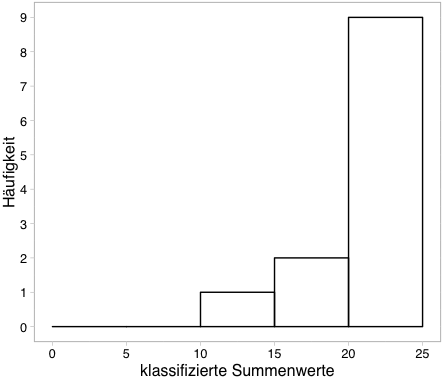
\includegraphics[width=0.8\linewidth]{Anhang/FKHistnn.png}

\end{minipage}
\begin{minipage}{.4\linewidth}
\centering
\raisebox{\depth}
{\begin{tabular}{rrrr}
  \hline
 & absolut & Prozent & kumuliert \\
  \hline
(0,5] & 0.00 & 0.00 & 0.00 \\
  (5,10] & 0.00 & 0.00 & 0.00 \\
  (10,15] & 1.00 & 8.33 & 8.33 \\
  (15,20] & 2.00 & 16.67 & 25.00 \\
  (20,25] & 9.00 & 75.00 & 100.00 \\
   \hline
\end{tabular}

}
%\caption{Häufigkeitstabelle: Fachkompetenz}
%\label{tab:defis}
\end{minipage}
\caption{Histogramm und Häufigkeitstabelle der Fachkompetenz}
\label{FK}
\end{figure}

Die Lagemaße der Fachkompetenz (Tabelle \ref{tab:lFK}) ergeben einen
Mittelwert von ca. 21. Dieser sehr hohe Wert entspricht auch dem Median
und dem Modus, was auf eine gleichmäßige Verteilung der Daten schließen
lässt. Der niedrigste Wert lag bei 14 der höchste Wert bei 25.

\begin{table}[H]
\centering
\caption{Lage- und Streumaße Fachkompetenz}
\label{tab:lFK}
\begin{tabular}{rrrrrrrr}
  \hline
  N & Minimum & Maximum & Mittelwert & Median & Modus & SD & Varianz \\
  \hline
 12.00 & 14.00 & 25.00 & 20.58 & 21.00 & 21.00 & 3.03 & 9.17 \\
   \hline
\end{tabular}
\end{table}

\subsubsection{Methodenkompetenz}\label{methodenkompetenz}

Auch bei der Methodenkompetenz, siehe Abbildung \ref{fig:MK}, wird
mindestens ein mittlerer Zuwachs eingeschätzt (bei 50\% der Teilnehmer).
Fünf Teilnehmer schätzen ihren Zuwachs hier als hoch ein, ein Teilnehmer
auf sehr hoch.

\begin{figure}[H]
\begin{minipage}{.4\linewidth}
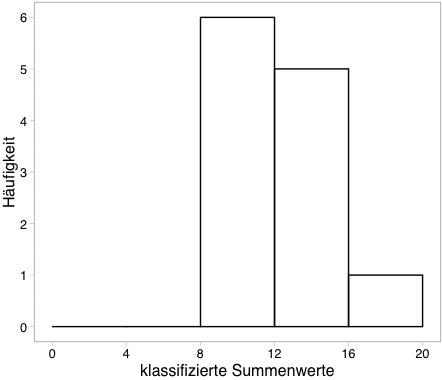
\includegraphics[width=0.8\linewidth]{Anhang/MKHistnn.png}


\end{minipage}
\begin{minipage}{.4\linewidth}
\centering
\raisebox{\depth}
{\begin{tabular}{rrrr}
  \hline
 & absolut & Prozent & kumuliert \\ 
  \hline
(0,4] & 0.00 & 0.00 & 0.00 \\ 
  (4,8] & 0.00 & 0.00 & 0.00 \\ 
  (8,12] & 6.00 & 50.00 & 50.00 \\ 
  (12,16] & 5.00 & 41.67 & 91.67 \\ 
  (16,20] & 1.00 & 8.33 & 100.00 \\ 
   \hline
\end{tabular}

}
%\caption{Häufigkeitstabelle: Fachkompetenz}
\label{tab:defis}
\end{minipage}
\caption{Histogramm und Häufigkeitstabelle der Methodenkompetenz}
\label{fig:MK}
\end{figure}

Wie Tabelle \ref{tab:lMK} zeigt kam der Wert 10 am häufigsten vor.
Mittelwert und Median liegen bei etwa 12.5, was gerade noch der Klasse
4, also hohem Kompetenzzuwachs entspricht. Der niedrigste Wert lag bei
10, der höchste Wert bei 17.

\begin{table}[H]
\centering
\caption{Lage- und Streumaße Methodenkompetenz}
\label{tab:lMK}
\begin{tabular}{rrrrrrrr}
  \hline
  N & Minimum & Maximum & Mittelwert & Median & Modus & SD & Varianz \\
  \hline
  12.00 & 10.00 & 17.00 & 12.83 & 12.50 & 10.00 & 2.41 & 5.79 \\
   \hline
\end{tabular}
\end{table}

\subsubsection{Personalkompetenz}\label{personalkompetenz}

Der Zuwachs an Personalkompetenz, siehe Abbildung \ref{fig:PK} wurde von
etwa zwei Drittel der Teilnehmer als hoch eingeschätzt, von einem
Teilnehmer als mittel und von 3 Teilnehmern als sehr hoch. Es gibt keine
Teilnehmer die keinen oder einen geringen personalen Kompetenzzuwachs
einschätzen.

\begin{figure}[H]
\begin{minipage}{.4\linewidth}
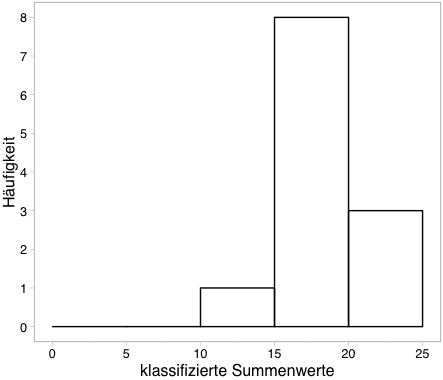
\includegraphics[width=0.8\linewidth]{Anhang/PKHistnn.png}

%\label{PK}
\end{minipage}
\begin{minipage}{.4\linewidth}
\centering
\raisebox{\depth}
{\begin{tabular}{rrrr}
  \hline
 & absolut & Prozent & kumuliert \\
  \hline
(0,5] & 0.00 & 0.00 & 0.00 \\
  (5,10] & 0.00 & 0.00 & 0.00 \\
  (10,15] & 1.00 & 8.33 & 8.33 \\
  (15,20] & 8.00 & 66.67 & 75.00 \\
  (20,25] & 3.00 & 25.00 & 100.00 \\
   \hline
\end{tabular}

}
%\caption{Häufigkeitstabelle: Fachkompetenz}
\label{tab:defis}
\end{minipage}
\caption{Histogramm und Häufigkeitstabelle der Personalkompetenz}
\label{fig:PK}
\end{figure}

Mittelwert, Median und Modalwert liegen bei 19, der kleinste Wert
beträgt 11 der höchste Wert 23 (Tabelle \ref{tab:lPK}). Zusammenfassend
betrachtet ist auch in dieser Kategorie der selbsteingeschätzte
Kompetenzzuwachs als hoch einzustufen.

\begin{table}[H]
\centering
\caption{Lage- und Streumaße: Personalkompetenz}
\label{tab:lPK}
\begin{tabular}{rrrrrrrr}
  \hline
  N & Minimum & Maximum & Mittelwert & Median & Modus & SD & Varianz \\
  \hline
  12.00 & 11.00 & 23.00 & 19.17 & 19.00 & 19.00 & 3.04 & 9.24 \\
   \hline
\end{tabular}
\end{table}

\subsubsection{Kommunikationskompetenz}\label{kommunikationskompetenz}

Der Zuwachs der Kommunikationskompetenz wird von einem Teilnehmer als
gering eingeschätzt, von den übrigen ca 90\% als mindestens mittel Etwa
50\% der Teilnehmer schätzen ihren Kompetenzzuwachs als hoch bis sehr
hoch ein (Abbildung \ref{fig:KK}).

\begin{figure}[H]
\begin{minipage}{.4\linewidth}
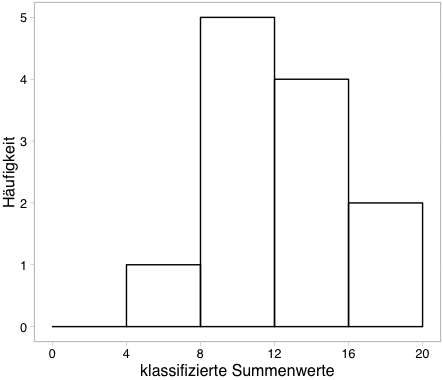
\includegraphics[width=0.8\linewidth]{Anhang/KKHistnn.png}

\label{pic:aufbau}
\end{minipage}
\begin{minipage}{.4\linewidth}
\centering
\raisebox{\depth}
{\begin{tabular}{rrrr}
  \hline
 & absolut & Prozent & kumuliert \\
  \hline
(0,4] & 0.00 & 0.00 & 0.00 \\
  (4,8] & 1.00 & 8.33 & 8.33 \\
  (8,12] & 5.00 & 41.67 & 50.00 \\
  (12,16] & 4.00 & 33.33 & 83.33 \\
  (16,20] & 2.00 & 16.67 & 100.00 \\
   \hline
\end{tabular}

}
%\caption{Häufigkeitstabelle: Fachkompetenz}
\label{tab:defis}
\end{minipage}
\caption{Histogramm und Häufigkeitstabelle der Kommunikationskompetenz}
\label{fig:KK}
\end{figure}

Der Zuwachs an Kommunikationskompetenz wurde von den Teilnehmern,
verhältnismäßig gering eingeschätzt. Der Mittelwert beträgt 13, der
Modalwert 12, damit kann der Zuwachs aber dennoch als gerade noch hoch
bewertet werden. Der niedrigste Wert ist 8, der höchste 18 (Tabelle
\ref{tab:lKK}).

\begin{table}[H]
\centering
\caption{Lage- und Streumaße: Kommunikationskompetenz}
\label{tab:lKK}
\begin{tabular}{rrrrrrrr}
  \hline
  N & Minimum & Maximum & Mittelwert & Median & Modus & SD & Varianz \\
  \hline
 12.00 & 8.00 & 18.00 & 13.00 & 12.50 & 9,11,16,18 & 3.54 & 12.55 \\

\end{tabular}
\end{table}

\subsubsection{Handlungskompetenz}\label{handlungskompetenz-1}

Für die Darstellung der Handlungskompetenzen werden die Werte der
einzelnen Kompetenzen addiert. Über 90\% der Teilnehmer schätzen ihren
Zuwachs an Handlungskompetenz als mindestens hoch ein, davon 25\% sogar
als sehr hoch. Ein Teilnehmer gibt lediglich einen mittleren Zuwachs an
(Abbildung \ref{fig:HK}).

\begin{figure}[H]
\begin{minipage}{.4\linewidth}
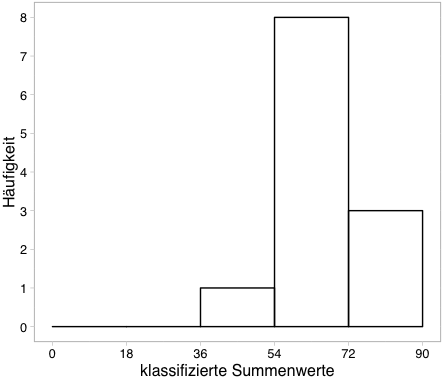
\includegraphics[width=0.8\linewidth]{Anhang/HKHistnn.png}

\label{pic:aufbau}
\end{minipage}
\begin{minipage}{.4\linewidth}
\centering
\raisebox{\depth}
{\begin{tabular}{rrrr}
  \hline
 & absolut & Prozent & kumuliert \\ 
  \hline
(0,18] & 0.00 & 0.00 & 0.00 \\ 
  (18,36] & 0.00 & 0.00 & 0.00 \\ 
  (36,54] & 1.00 & 8.33 & 8.33 \\ 
  (54,72] & 8.00 & 66.67 & 75.00 \\ 
  (72,90] & 3.00 & 25.00 & 100.00 \\ 
   \hline
\end{tabular}

}
%\caption{Häufigkeitstabelle: Fachkompetenz}
\label{tab:defis}
\end{minipage}
\caption{Histogramm und Häufigkeitstabelle der Handlungskompetenz}
\label{fig:HK}
\end{figure}

Der Mittelwert des Zuwachses an Handlungskompetenz beträgt etwa 65,
ebenso wie der Median. Es gibt zwei Modalwerte 63 und 75. Der niegrigste
Wert lag bei 44 der höchste Wert bei 75 (Tabelle \ref{lHK}).

\begin{table}[H]
\centering
\caption{Lage- und Streumaße der Handlungskompetenz}
\label{lHK}
\begin{tabular}{rrrrrrrr}
  \hline
  N & Minimum & Maximum & Mittelwert & Median & Modus & SD & Varianz \\
  \hline
12.00 & 44.00 & 75.00 & 65.58 & 65.50 & 63,75 & 8.49 & 72.08 \\
   \hline
\end{tabular}
\end{table}

Die dicht zusammenliegenden Werte der zentralen Tendenz deuten darauf
hin, dass die Verteilung der Werte gleichmäßig ist. Die Streuung der
Werte um den Mittelwert ist bei der Kommunikationskompetenz am größten
und bei der Methodenkompetenz am kleinsten. Der Zuwachs an Fachkompetenz
wurde im Mittel als sehr hoch eingeschätzt, der Zuwachs der anderen
Kompetenzen als hoch.

\subsubsection{Nutzungsverhalten}\label{nutzungsverhalten}

Beim Nutzungsverhalten wird sowohl die Intensität, als auch die Art der
Nutzung abgefragt. Es gibt zum Nutzungsverhalten 8 Items, die jeweils
mit der Angabe der Häufigkeit 0-1, 2-4, 5-7, 8-10 oder \textgreater{} 10
mal beantwortet werden können. Die Plattform wurde von 5 Teilnehmern
wenig, von 7 Teilnehmern etwas mehr genutzt. Die Klassen keine Nutzung,
häufige und sehr häufige Nutzung kommen nicht vor (Abbildung
\ref{fig:NV}).

\begin{figure}[H]
\begin{minipage}{.4\linewidth}
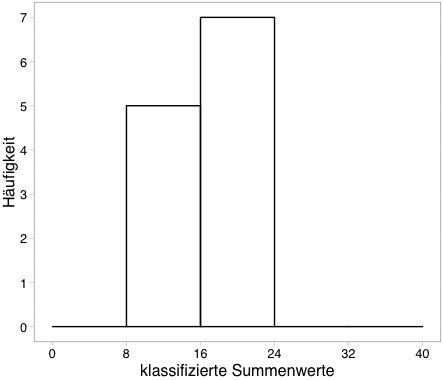
\includegraphics[width=0.8\linewidth]{Anhang/NVHistnn.png}

\label{pic:aufbau}
\end{minipage}
\begin{minipage}{.4\linewidth}
\centering
\raisebox{\depth}
{\begin{tabular}{rrrr}
  \hline
 & absolut & Prozent & kumuliert \\ 
  \hline
(0,8] & 0.00 & 0.00 & 0.00 \\ 
  (8,16] & 5.00 & 41.67 & 41.67 \\ 
  (16,24] & 7.00 & 58.33 & 100.00 \\ 
  (24,32] & 0.00 & 0.00 & 100.00 \\ 
  (32,40] & 0.00 & 0.00 & 100.00 \\ 
   \hline
\end{tabular}

}
%\caption{Häufigkeitstabelle: Fachkompetenz}
\label{tab:defis}
\end{minipage}
\caption{Histogramm und Häufigkeitstabelle des Nutzungsverhaltens}
\label{fig:NV}
\end{figure}

Die Lernplattform wurde nur wenig genutzt (Tabelle \ref{fig:NV}):
Durchschnittlich bewegt sich die Nutzung des digitalen Angebotes mit
17.55 in einem mittleren Bereich. Die Bimodulare Verteilung (14 und 19)
weist auf nicht normalverteilte Daten hin. Die niedrigsten und höchsten
Werte liegen zwischen 9 und 21.

\begin{table}[H]
\centering
\caption{Lage- und Streumaße: Nutzungsverhalten}
\label{tab:NV}
\begin{tabular}{rrrrrrrr}
  \hline
  N & Minimum & Maximum & Mittelwert & Median & Modus & SD & Varianz \\
  \hline
 12.00 & 9.00 & 21.00 & 16.42 & 17.50 & 14,19 & 3.32 & 10.99 \\     
   \hline
\end{tabular}
\end{table}

\subsection{Bivariate Auswertung}\label{bivariate-auswertung}

\subsubsection{Handlungskompetenz und Nutzungsverhalten
allgemein}\label{handlungskompetenz-und-nutzungsverhalten-allgemein}

Es soll nun weiter untersucht wurde welchen Einfluss die Nutzung der
Lernplattform auf dem Kompetenzzuwachs hat. Dazu werden der
Gesamtkompetenzzuwachs (abhängige Variable) und die Nutzungshäufigkeit
(unabhängige Variable) in einem Streudiagramm gegeneinander aufgetragen.
Ob es eine Abhängigkeit zwischen den Variablen gibt wird mit dem
Spearmans rho Test überprüft. Dieser Test wird gewählt, da er für
kleine, nichtnormalverteilte Datenmengen am ehesten geeignet ist.
\improvement{hier noch ein Zitat}

\begin{figure}[H]
\centering
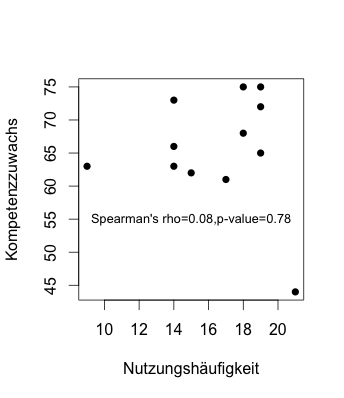
\includegraphics[width=0.33\textwidth]{Anhang/Spearman.png}
\caption{Kompetenzzuwachs und Nutzung, mit Ergebnis von Spearman rho}
\label{fig:spear}
\end{figure}

Im Streudiagramm (Abbildung \ref{fig:spear}) wird deutlich, dass es
keine Abhängigkeit zwischen den Variablen gibt. Der rho-Wert 0,08 bei
einem p-Wert von 0,78 zeigt ebenfalls, dass es keinen Zusammenhang gibt.

\subsubsection{Handlungskompetenz und
Nutzungsart}\label{handlungskompetenz-und-nutzungsart}

Mit dem Fragebogen wurde zum einen die Nutzungsintensität und zum
anderen die Art der Nutzung abgefragt. Dabei gibt es passive Formen der
Nutzung: Termininformation, Beiträge lesen, Fotos anschauen, Dateien
nutzen und aktive Formen der Nutzung: Beiträge in Forum und Glossar
verfassen, am Lernquiz teilnehmen. Die Aufteilung des Nutzungsverhalten
in aktive (Item 1-5) und passive Nutzung (6-8) zeigen auch getrennt
betrachtet keine Abhängigkeit zum Zuwachs an Handlungskompetenz (Anhang
\ref{sec:aktiv}). Auf eine weitere Zerlegung der Daten wird aufgrund der
sehr kleinen Datenmenge verzichtet. Das heißt, die Abhängigkeiten auf
die unterschiedlichen Kompetenzen, finden hier keine Berücksichtigung.

\section{Diskussion und Fazit}\label{diskussion-und-fazit}

Hypothese 1: Die Teilnahme an der Weiterbildungsmaßnahme führt deutlich
zu einem Zuwachs an selbsteingeschätzter Handlungskompetenz, d.h. die
Nullhypothese wird verworfen. Hypothese 2: Die Nutzungsintensität der
Lernplattform hat keinen Einfluss auf den Kompetenzzuwachs, d.h. die
Nullhypothese wird angenommen Zusammenfassend lässt sich die
vorangestellte Forscherfrage wie folgt beantworten: Der Blended Learning
Kurs „Umsetzung des Bildungs- und Orientierungsplans in der
Kindertagesstätte mit dem Early Excellence-Konzept`` fördert den Zuwachs
der Kompetenzen, unabhängig von der Nutzung der Lernplattform.\\
Am höchsten wurde, wie zu Erwarten der Zuwachs an Fachkompetenz
eingeschätzt, denn es wurde viel Fachwissen „gelehrt``. Der Zuwachs an
Methoden-, Personal- und Kommunikationskompetenz ist im Vergleich dazu
geringer, da hier auch schon individuell mehr an Vorwissen vorhanden
ist.

Wie die Ergebnisse zeigen, wurde die Lernplattform nicht sehr intensiv
genutzt und es ist kein Einfluss auf den Zuwachs sichtbar. Allerdings
muss hier angemerkt werden, dass die Form des digitalen Lernens für
viele Teilnehmer eine sehr neue Erfahrung war und der
selbstverständliche Umgang damit noch nicht gegeben ist. Ein weiterer
wichtiger Aspekt ist der Umgang mit Zeit: während die Präsenztage
gutgeschrieben werden, erstreckt sich die Nutzung der Lernplattform auf
Freizeit. Auch wenn es sich hier in Zahlen nicht ausdrücken lässt, so
lassen die Kommentare im freien Textfeld den Schluss zu, dass die
Lernplattform einen gleich wie gerichteten, positiven Effekt auf den
Nutzer hat: „Ich finde die Lernplattform super! Auch die schnelle
Verbindung zu allen Teilnehmern finde ich gut. Sie ist wirklich eine
große Hilfe, weil man alles auf einen Blick und sehr übersichtlich
hat.``

Die vorliegende Forschungsarbeit hat das Ziel, eine berufliche
Weiterbildungsmaßnahme im Blended Learning Format zu evaluieren. Inhalt
der Weiterbildung ist das Early Excellence-Konzept und seine Umsetzung
in der Kindertagesstätte. Da es in der Erwachsenenbildung allgemein
vielmehr um das Erreichen von Handlungskompetenz als um die bloße
Vermehrung von Wissen geht, wurde der Versuch unternommen, den Zuwachs
an Handlungskompetenz zu messen. Dies wurde, entsprechend der Literatur,
mittels eines Fragebogens zur Selbsteinschätzung umgesetzt. Die
Ergebnisse zeigen, dass die Teilnehmer den Effekt auf den Zuwachs an
unterschiedlichen Kompetenzen als hoch einschätzen. Die Ergebnisse
zeigen allerdings auch, dass die Nutzung der Lernplattform keinen
Einfluss auf dieses Zuwachs zu haben scheint. Die Ergebnisse dieser
Arbeit sind allerdings erheblichen Einschränkungen unterworfen. Die
Datenmenge ist mit n=12 extrem klein und die Ergebnisse sind daher nicht
übertragbar oder gar zu verallgemeinern. Um die digitale Nutzung zu
intensivieren ist eventuell mehr Zeit erforderlich, da die
Auseinandersetzung mit der Technik nicht von allen so schnell geleistet
werden kann. Abhilfe könnte hier eine noch engere Verknüpfung von
Präsenzphasen und digitalem Lernen schaffen: Beispielsweise könnte die
Lernplattform auch während den Präsenzphasen genutzt werden oder die
Präsenzzeiten zugunsten der digitalen Lernzeit verkürzt werden. Denn
besonderes in beruflichen Weiterbildungen, wo Zeit ein sehr knappes Gut
ist, kann das zeit- und ortsunabhängige Lernen, dass durch digitale
Lernplattformen ermöglicht wird, ein großer Zugewinn sein.
\change{Literaturverzeichnis!}

\pagebreak
\printbibliography
\section{Erklärung}
\centering
\makebox[0pt]
{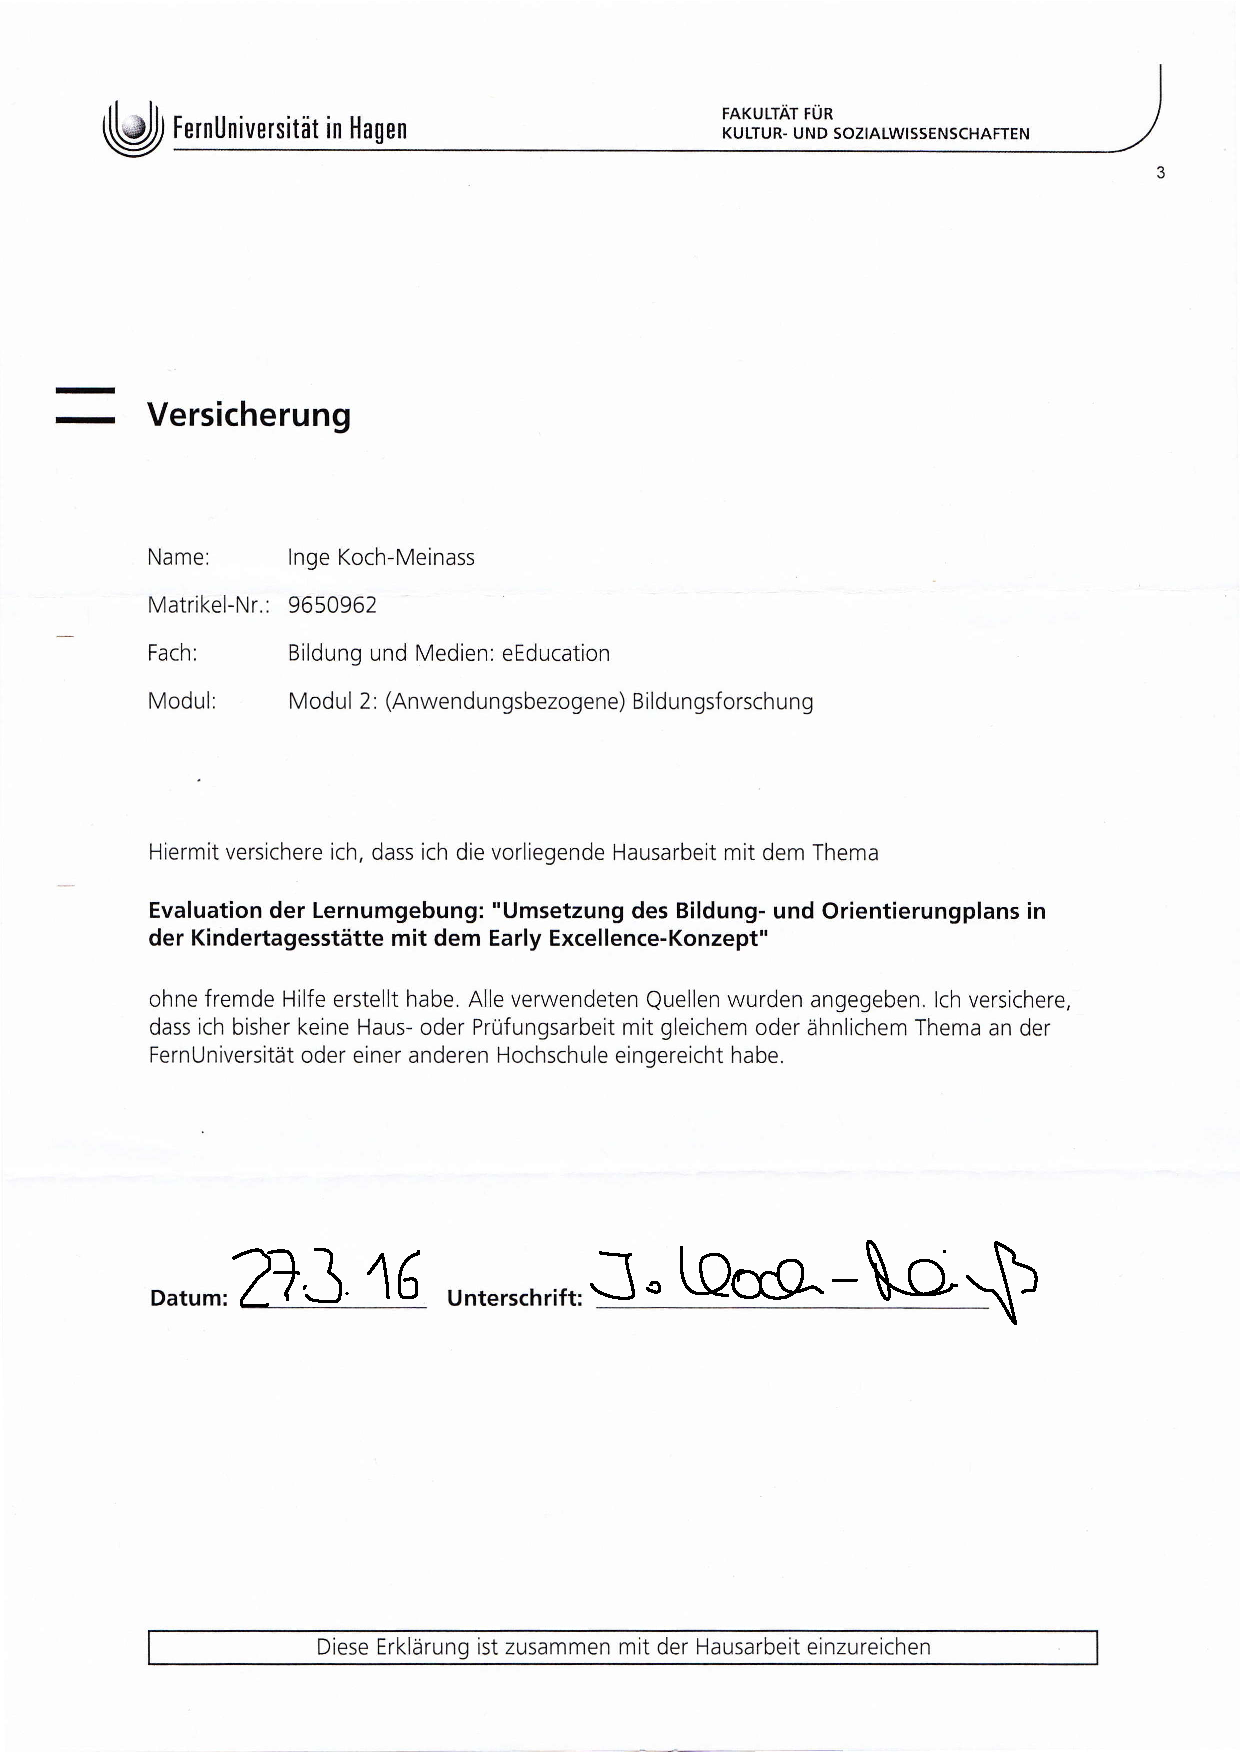
\includegraphics[scale=0.65]{Anhang/erklaerunghausarbeit.pdf}}

\pagebreak
\appendix


  \section{Anhang}
  \subsection{Ergebnisse: Cronbach's alpha}
  \label{sec:cron}
  %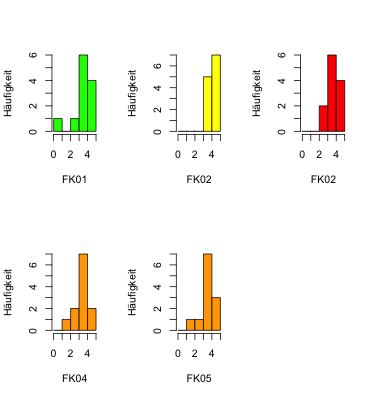
\includegraphics{Anhang/schoen.png}
  %\subsection{Abkürzungen}
  %\renewcommand{\thetable}{{A}.\arabic{table}}
  %\renewcommand{\thetable}{\Alph{section}.\arabic{table}}
  \begin{table}[H]
\centering
%\caption{Ergebnisse: Cronbach's alpha}
%\label{cronbach}
\begin{tabular}{@{}lll@{}}
\toprule
Kompetenz               & Cronbachs alpha & Items               \\ \midrule
Fachkompetenz           & 0.84            & FK1,FK2,FK3,FK4,FK5 \\
Methodenkompetenz       & 0.73            & MK1,MK2,MK3,MK4     \\
Personalkompetenz       & 0.91            & PK1,PK2,PK3,PK4,PK5 \\
Kommunikationskompetenz & 0.93            & KK1,KK2,KK3,K4      \\ \bottomrule
\end{tabular}
\end{table}
  \subsection{Itemzuordnung}
  \label{sec:item}
  \begin{table}[H]
\centering
%\captionof{table}[Anhang]{Titel}
%\caption{Zuordnung der Items}
\label{itemtabelle}
\resizebox{\textwidth}{!}{%
\begin{tabular}{@{}lllll@{}}
\toprule
Item  & Konstrukt                                                                    & Indikator                                                                                                                                                                           & Ausprägung                                                                                                                                                                                       & Skalenniveau \\ \midrule
1-5   & \begin{tabular}[c]{@{}l@{}}Fach-\\ kompetenz\\FK1,FK2,FK3,FK4,FK5\end{tabular}                    & \begin{tabular}[c]{@{}l@{}}Disposition sachlich-gegenständliche\\ Probleme selbstorganisiert lösen zu können\end{tabular}                                                           & \begin{tabular}[c]{@{}l@{}}5-stufige Likertskala:\\ 1= trifft überhaupt nicht zu\\ 2= trifft wenig zu\\ 3=trifft teils/teils zu\\ 4=trifft überwiegend zu\\ 5=trifft völlig zu\end{tabular}      & metrisch     \\
\midrule
6-10  & \begin{tabular}[c]{@{}l@{}}Methoden-\\ kompetenz\\MK1,MK2,MK3,MK4\end{tabular}                & \begin{tabular}[c]{@{}l@{}}Tätigkeiten und Aufgaben methodisch\\  selbst-organisiert zu gestalten und Methoden\\  weiter zu entwickeln\end{tabular}                                 & \begin{tabular}[c]{@{}l@{}}5-stufige Likertskala: \\ 1= trifft überhaupt nicht zu\\ 2= trifft wenig zu \\ 3=trifft teils/teils zu \\ 4=trifft überwiegend zu \\ 5=trifft völlig zu\end{tabular}  & metrisch     \\
\midrule
11-16 & \begin{tabular}[c]{@{}l@{}}Personal-\\ kompetenz\\PK1,PK2,PK3,PK4,PK5\end{tabular}                & \begin{tabular}[c]{@{}l@{}}Sich einschätzen, selbstorganisiert reflexiv\\  handeln,Werte, Motive und Selbstbilder\\  entwickeln\end{tabular}                                        & \begin{tabular}[c]{@{}l@{}}5-stufige Likertskala: \\ 1= trifft überhaupt nicht zu \\ 2= trifft wenig zu \\ 3=trifft teils/teils zu \\ 4=trifft überwiegend zu \\ 5=trifft völlig zu\end{tabular} & metrisch     \\
\midrule
17-21 & \begin{tabular}[c]{@{}l@{}}Komunikations-\\ kompetenz\\KK1,KK2,KK3,KK4\end{tabular}           & \begin{tabular}[c]{@{}l@{}}Sich mit anderen kreativ auseinander setzen, \\ kommunikativ und selbstorganisiert handeln\\ \parencite[8]{ErpenbeckRosenstiel200305}\end{tabular} & \begin{tabular}[c]{@{}l@{}}5-stufige Likertskala\\ 1= trifft nicht zu,\\2= trifft wenig zu \\ 3=trifft teils/teils zu \\ 4=trifft überwiegend zu \\ 5=trifft vollständig zu\end{tabular}                                                                                    & metrisch     \\
 \midrule
22-28 & \begin{tabular}[c]{@{}l@{}}Nutzungs\\ verhalten\\ Lernplattform NV1,NV2,NV3\\NV4,NV5,NV6,NV7,NV8\end{tabular} & \begin{tabular}[c]{@{}l@{}}Aufschluss über die Intensität u\\ der Nutzung der Lernplattform\end{tabular}                                                                 & \begin{tabular}[c]{@{}l@{}}5-stufige Skala\\ 1=0-1mal genutzt\\ 2=2-4 mal genutzt\\ 3=5-7 mal genutzt\\ 4=8-10 mal genutzt\\ 5=\textgreater10 mal genutzt\end{tabular}                            & metrisch     \\ \bottomrule
\end{tabular}%
}
\end{table}

  \subsection{Einteilung der Klassen}
  \label{sec:klasse}
  \begin{table}[]
\centering
\caption{Einteilung der Klassen}
\label{tab:klassen}
\begin{tabular}{@{}llll@{}}
\toprule
Kompetenz              & Summenwert & Klasse & Bewertung          \\ \midrule
Fach/Personal          & 0-5        & 1      & kein Zuwachs       \\
                       & 5-10       & 2      & geringer Zuwachs   \\
                       & 10-15      & 3      & mittlerer Zuwachs  \\
                       & 15-20      & 4      & hoher Zuwachs      \\
                       & 20-25      & 5      & sehr hoher Zuwachs \\ \cmidrule(r){1-4}
Methoden/Kommunikation & 0-4        & 1      & kein Zuwachs       \\
                       & 4-8        & 2      & geringer Zuwachs   \\
                       & 8-12       & 3      & mittlerer Zuwachs  \\
                       & 12-16      & 4      & hoher Zuwachs      \\
                       & 16-20      & 5      & sehr hoher Zuwachs \\ 
                       \cmidrule(r){1-4}
Handlungskompetenz 	& 0-18       & 1      & kein Zuwachs       \\
                       & 18-36        & 2      & geringer Zuwachs   \\
                       & 36-54       & 3      & mittlerer Zuwachs  \\
                       & 54-72      & 4      & hoher Zuwachs      \\
                       & 72-90      & 5      & sehr hoher Zuwachs \\ 
                       \cmidrule(r){1-4}
Nutzung	& 0-8       & 1      & keine Nutzung       \\
                       & 8-16        & 2      & geringe Nutzung   \\
                       & 16-24       & 3      & mittlere Nutzung  \\
                       & 24-32     & 4      & häufige Nutzung      \\
                       & 32-40      & 5      & sehr häufige Nutzung \\ 
                       \bottomrule
\end{tabular}
\end{table}

  \subsection{Kompetenzzuwachs und Form der Nutzung}
  \label{sec:aktiv}
  \begin{figure}[H]
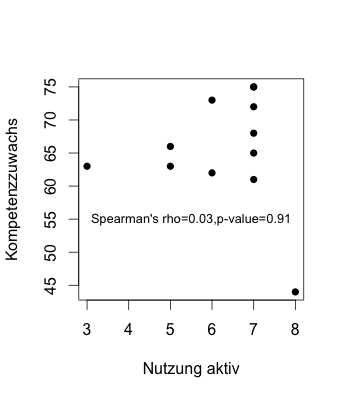
\includegraphics[width=0.4\linewidth]{Anhang/spearaktiv.png}
%\caption{Kompetenzzuwachs und aktive Nutzung}
%\label{fig:saktiv}
\end{figure}
%\subsection{Kompetenzzuwachs und passive Nutzung}
\begin{figure}[H]
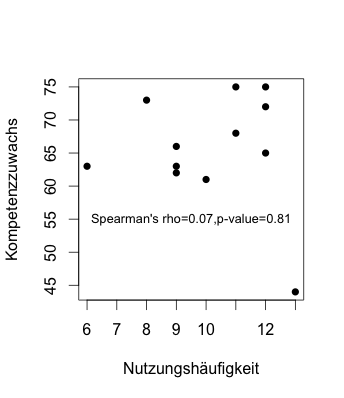
\includegraphics[width=0.4\linewidth]{Anhang/speerpassiv.png}
%\caption{Kompetenzzuwachs und passive Nutzung}
%\label{fig:spassiv}
\end{figure}
%\pagebreak
\subsection{Fragebogen}
\label{sec:fragen}

%\begin{figure}[H]
\centering
\makebox[0pt]
{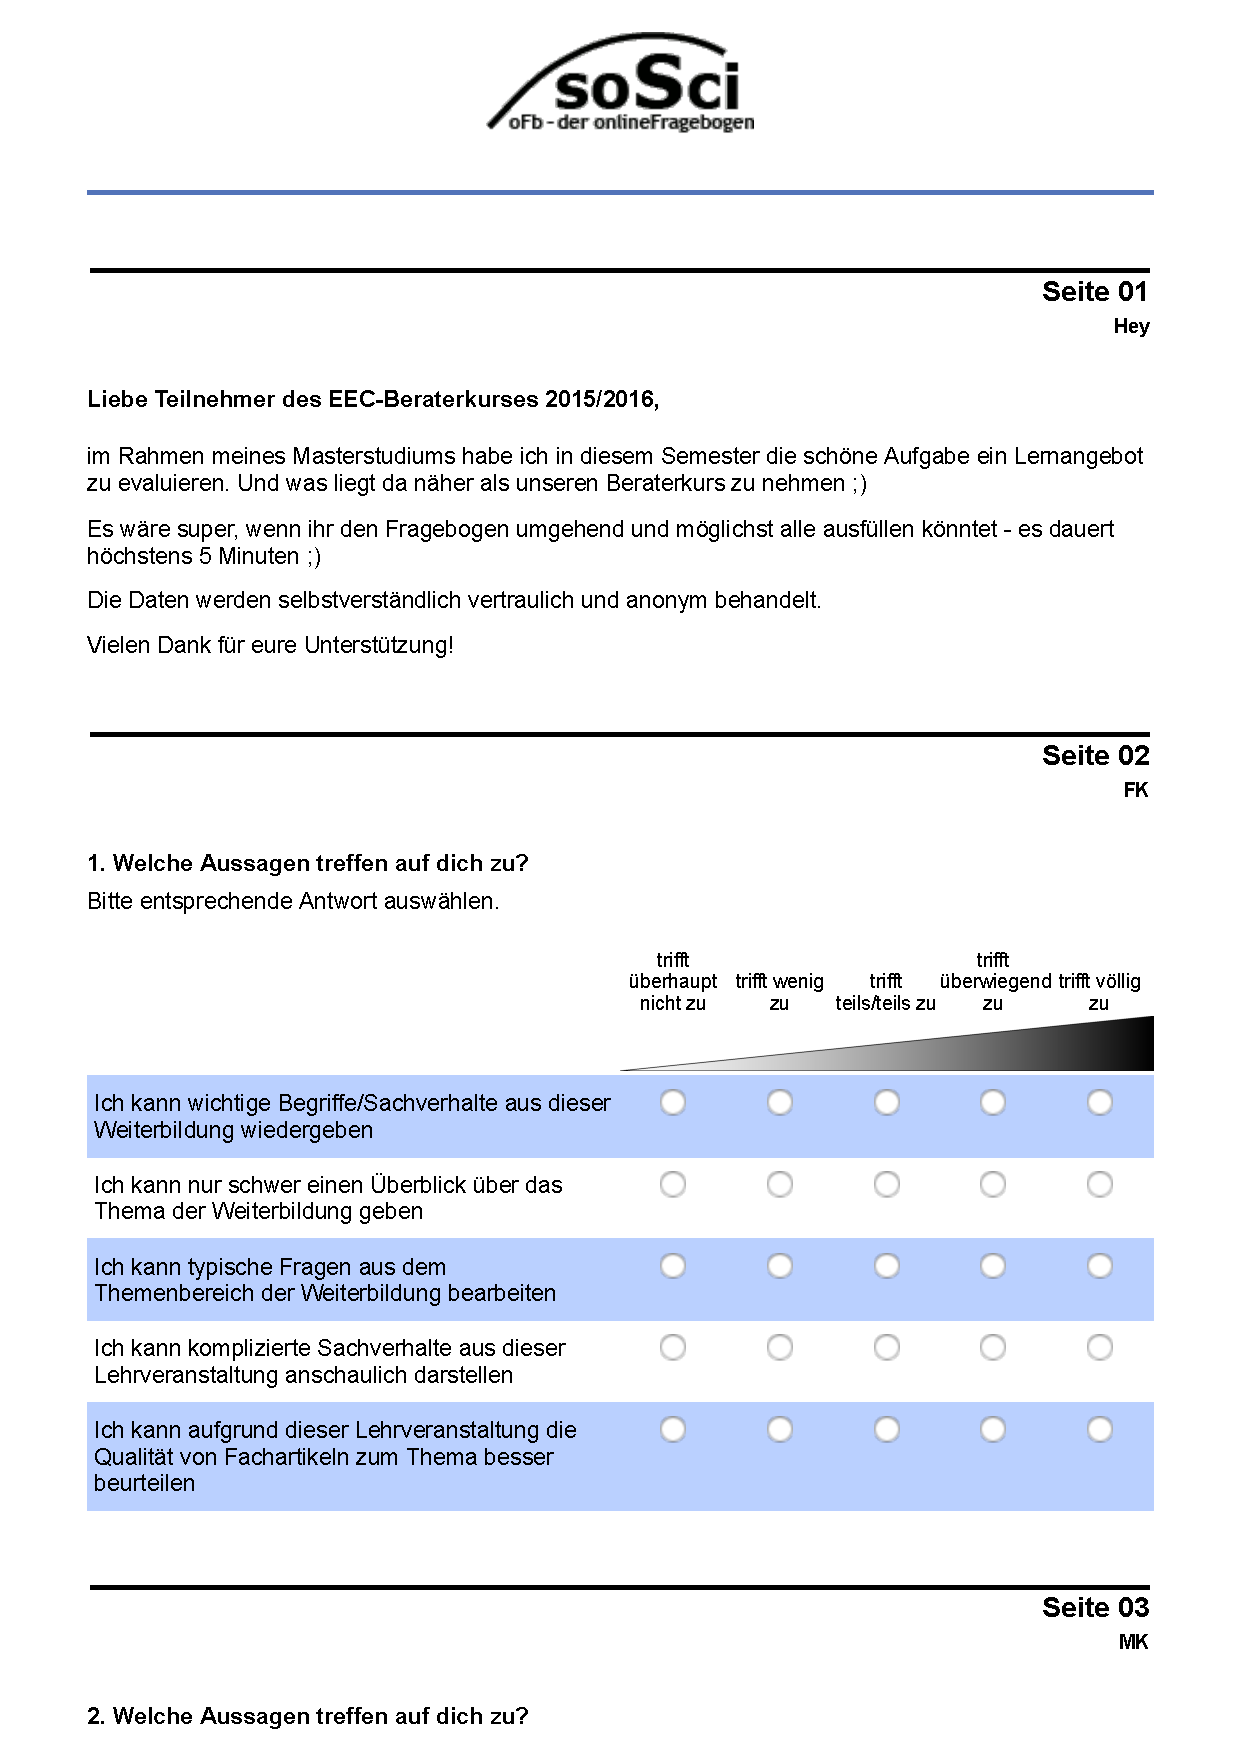
\includegraphics[scale=0.5]{Anhang/Fragebogen.pdf}}
%\end{figure}
\includepdf[pages=2-3,scale=0.7,pagecommand={\thispagestyle{headings}}]{Anhang/Fragebogen.pdf}

%\section{Erklärung}
%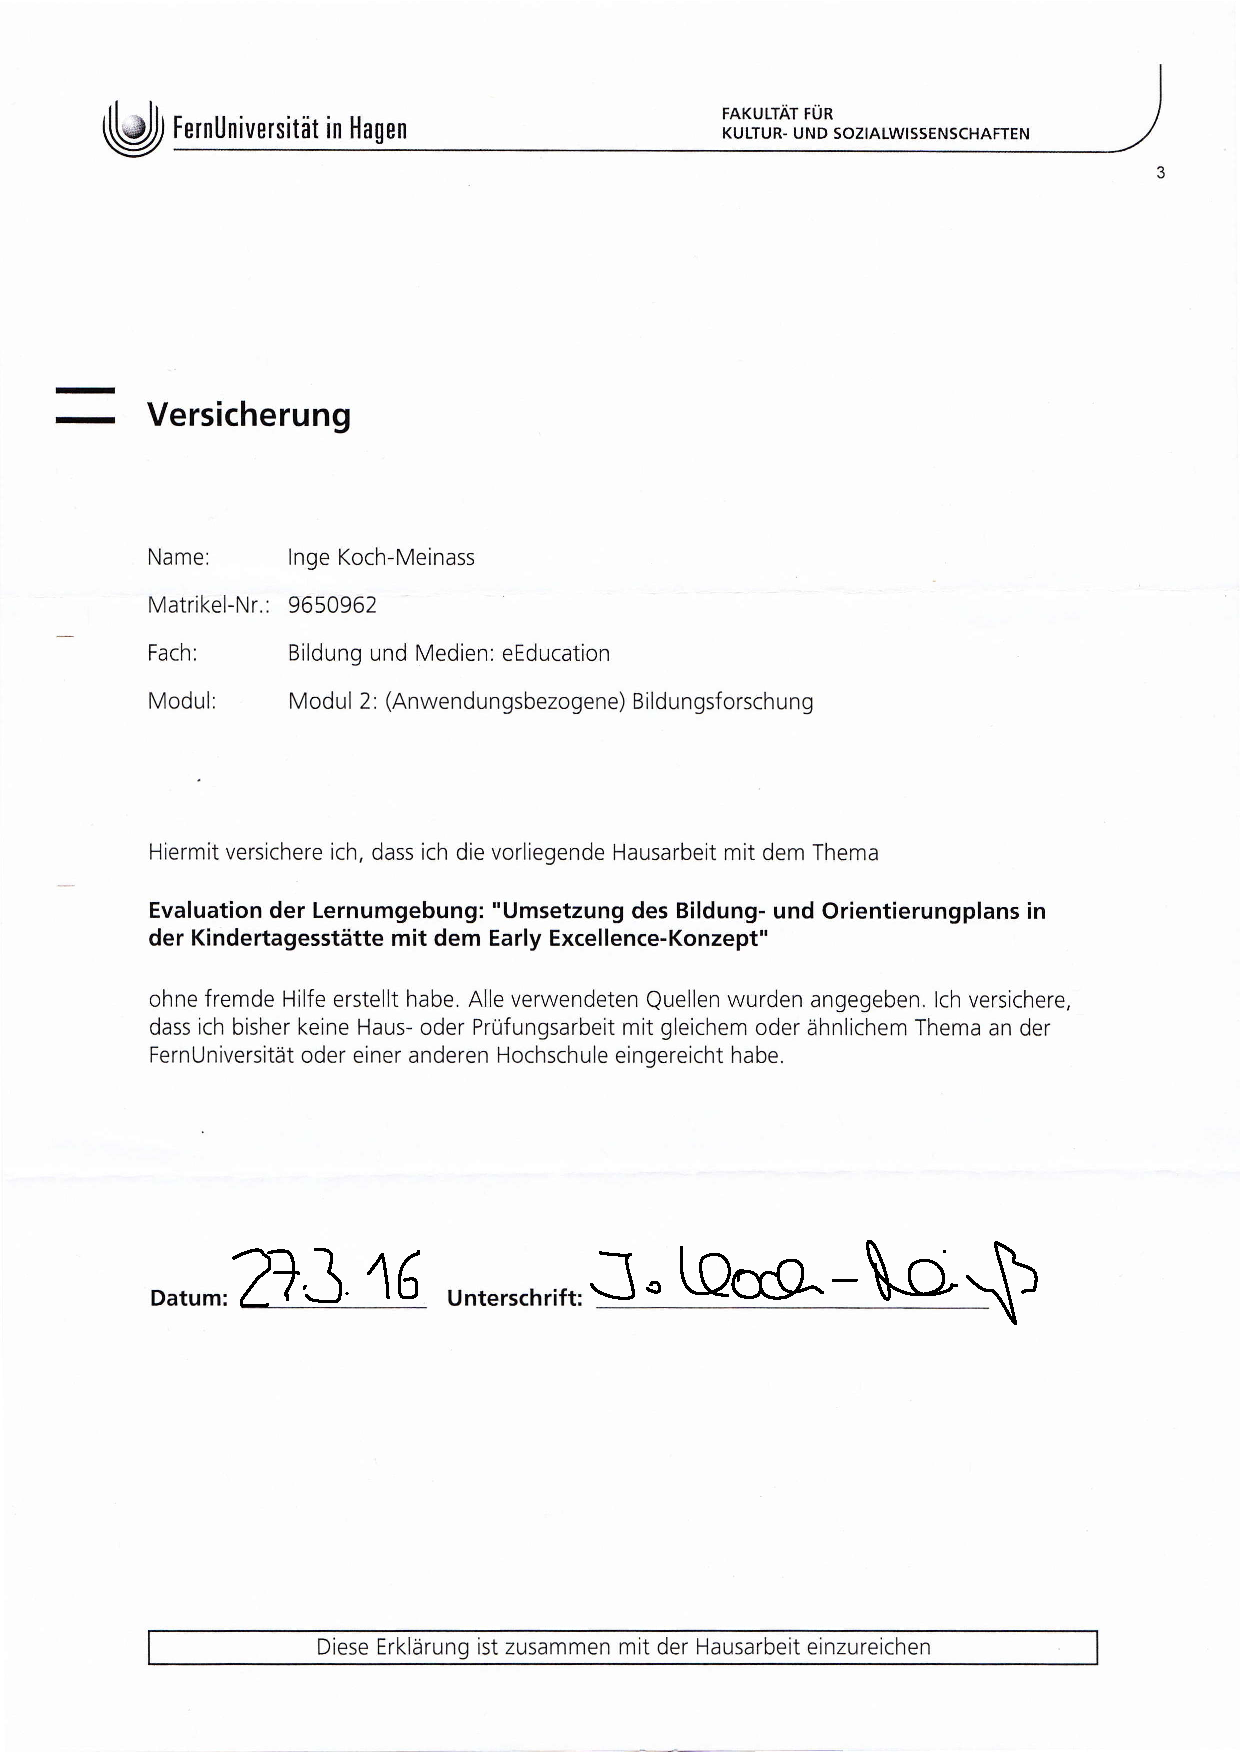
\includepdf{Anhang/erklaerunghausarbeit.pdf}
%\input{tabelleanalysen}
%\includepdf{alleine.pdf}
\end{document}
